\parx
Figure \ref{fig:cn_node_interface} shows the node interface that serves as the
workspace for the users to code visually by creating and managing nodes and
connections. The figure shows an example of a basic visual program.

\begin{figure}[H]
	\centering
	\captionsetup{justification=centering}
	\captionsetup[figure]{list=yes}
	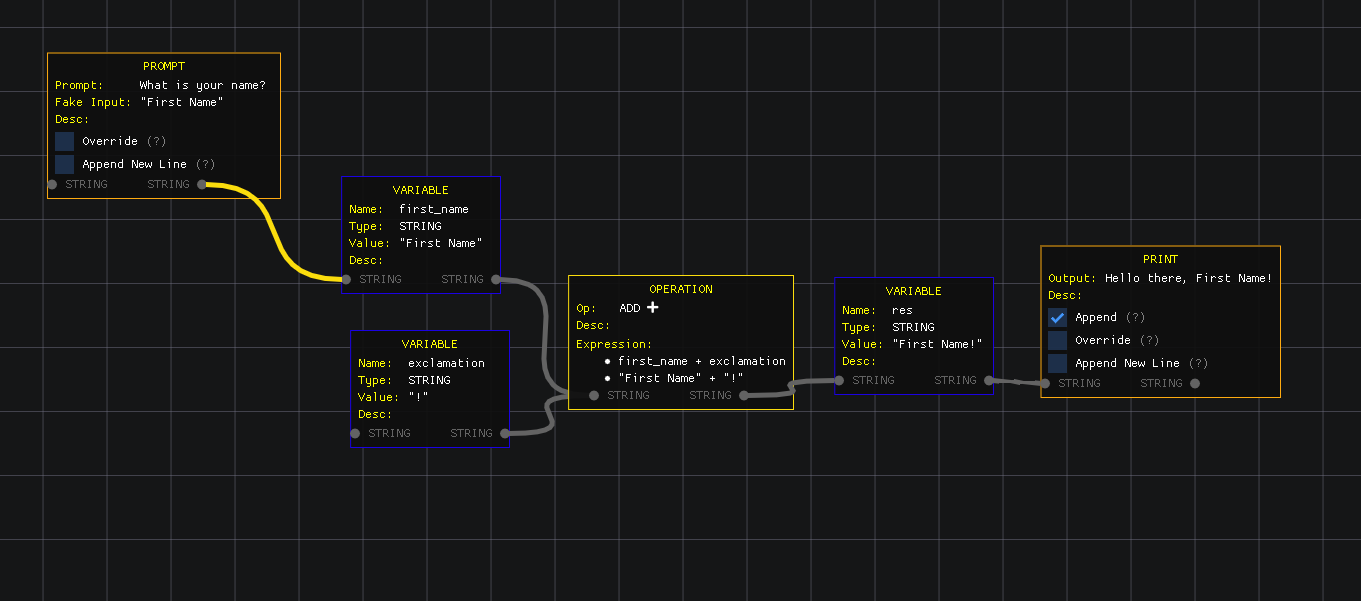
\includegraphics[width=\linewidth]{media/sc_node_interface.png}
	\caption[Node Interface of CodeNect]{Node Interface of CodeNect}
	\label{fig:cn_node_interface}
\end{figure}

\parx
Figure \ref{fig:cn_node_context} shows the node interface context menu that
lists all the possible kind of nodes, arranged by category, that the user can
create. The context menu can be opened by right-clicking anywhere on an empty
space on the node interface.

\begin{figure}[H]
	\centering
	\captionsetup{justification=centering}
	\captionsetup[figure]{list=yes}
	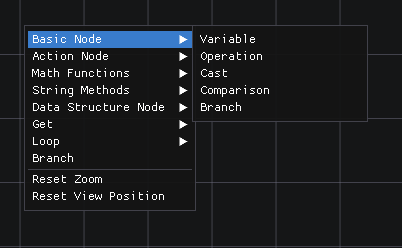
\includegraphics[width=\linewidth]{media/sc_node_interface_context.png}
	\caption[Node Interface Context Menu in CodeNect]{Node Interface Context Menu in CodeNect}
	\label{fig:cn_node_context}
\end{figure}

\parx
Figure \ref{fig:cn_node_create} shows a window for creating a node of kind
variable with the base required data such as name, data type, value, and a
conditional field for description or comment.

\begin{figure}[H]
	\centering
	\captionsetup{justification=centering}
	\captionsetup[figure]{list=yes}
	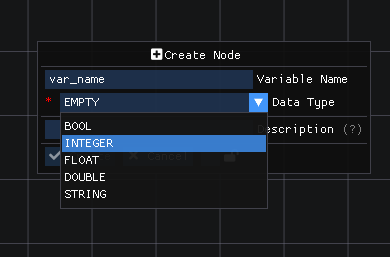
\includegraphics[width=\linewidth]{media/sc_node_creation_sample.png}
	\caption[Node Creation Sample in CodeNect]{Node Creation Sample in CodeNect}
	\label{fig:cn_node_create}
\end{figure}
